\fontsize{12}{12}\selectfont
\chapter{CAPITULO 3}
\section{Selecci�n de la herramienta para Data Discovery}
Fue analizado el Cuadrante M�gico de Gartner[REF] para la selecci�n de la mejor herramienta que se adecue a los criterios necesarios para ser utilizado en esta tesis.

\subsection{Cuadrante M�gico de Gartner}
\textsc{\begin{figure}[H]
	\centering
	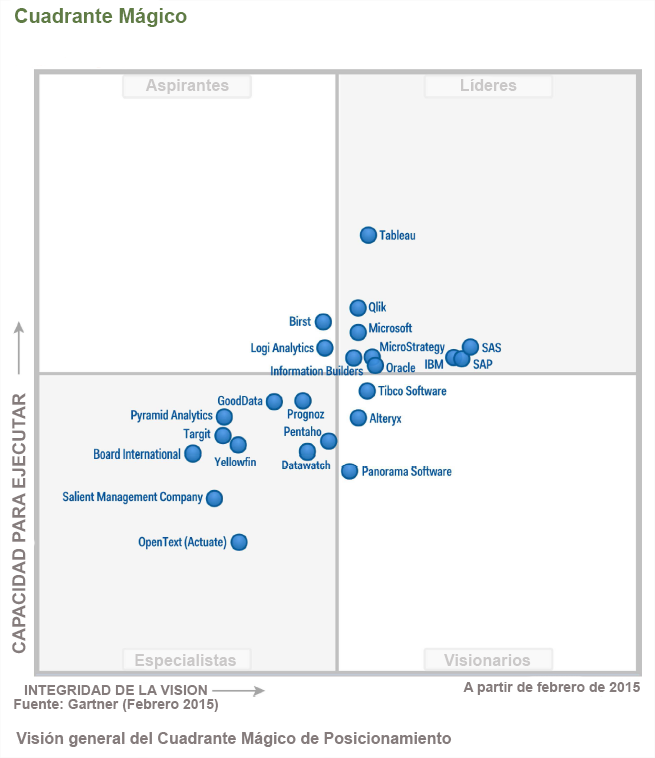
\includegraphics[width=160mm]{Magic-Quadrant.png}
	\caption{Cuadrante M�gico para BI y Plataformas Anal�ticas}
	\label{fig:magicQuadrant}
\end{figure}}

\subsection{Tableau}
Tableau tiene una posici�n fuerte en capacidad de ejecuci�n en el eje de l�deres del cuadrante. La herramienta Tableau fue la que mejor se adecu� a las necesidades del trabajo de Tesis, dado que cuenta con una versi�n P�blica para la construcci�n y publicaci�n de dashboards, adem�s de la facilidad de uso que nos proporciona. Tableau Desktop, la cual se basa en tecnolog�a drag and drop (arrastrar y soltar) permite analizar datos r�pidamente y le permite ver los cambios en tiempo real sin necesidad de codificaci�n.




\textsc{\begin{figure}[H]
	\centering
	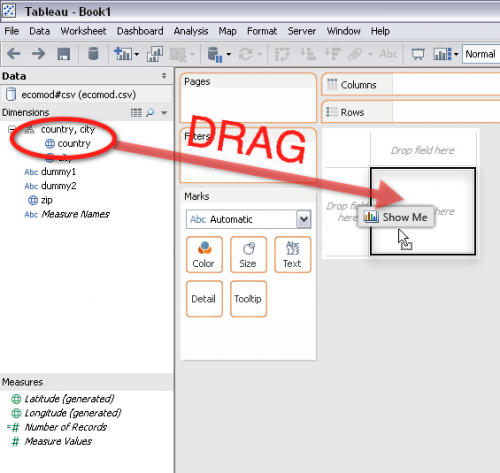
\includegraphics[width=0.7\linewidth]{figuras/tableauDragAndDrop2}
	\caption{Arrastre el campo pa�s para el campo desplegable se�alado.}
	\label{fig:tableauDragAndDrop2}
\end{figure}}



\textsc{\begin{figure}[H]
	\centering
	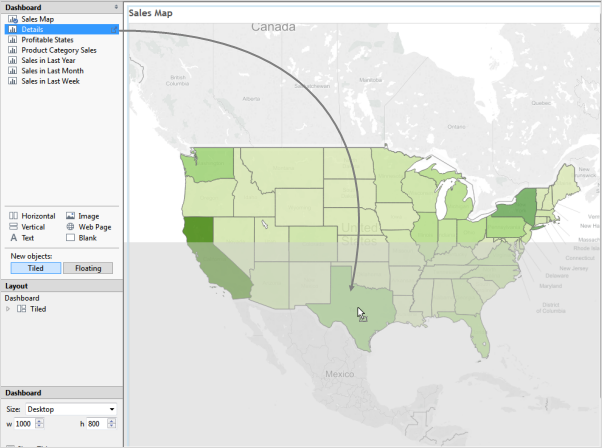
\includegraphics[width=0.7\linewidth]{figuras/tableauDragAndDrop1}
	\caption{Arrastrar hojas de trabajo al dashboard.}
	\label{fig:tableauDragAndDrop1}
\end{figure}}


En pocos pasos el usuario puede conectarse a diversas fuentes de datos y crear dashboards interactivos, conectando entre s� los diferentes componentes (tipo de gr�fico) que nos proporciona la herramienta, si as� se desea. Esto quiere decir que la herramienta permite utilizar un gr�fico como filtro para otro siendo o no de la misma fuente de datos.

En las empresas la utilizan para entender r�pidamente distintos aspectos de sus negocios. Tambi�n podr�an utilizar para realizar proyecciones o tendencias basada en estad�sticas,  la cual tableau nos ofrece estos c�lculos de manera autom�tica.